\section{Policy-compliant Resiliency}
Datacenter networks are highly prone to failures, 
and it is crucial to ensure certain guarantees during such failure
situations. For example, if the operator want to guarantee
reachability amongst endpoints, the controller has to find a active
path in the network to re-establish reachability. However
satisfying tenant SLAs like isolation after a failure occurs
can be prohibitively time-consuming due to the higher complexity
of enforcing policies. 
Thus, we propose a \emph{proactive} approach 
to \emph{policy-compliant resiliency} to tackle network failures
by synthesizing resilient data planes such that in the event
of certain failures, there exists a path for each class which satisfies
all input policies. 

In the section, we describe the transformation of input 
policies to provide $t-resilience$, i.e in the event of upto arbitary
$t$ link failures, \name will synthesize a path for each
packet class. We only consider reachability, waypoint
and isolation policies in the input. 

%\begin{mydef}
%	$t-resilience$ synthesis for a packet class is defined as the
%	synthesis of paths such that in the event of upto arbitary
%	$t$ link failures, there exists a synthesized path for the packet class which
%	satisfies the input policies. 
%\end{mydef}
\begin{mydef}
Given the physical topology $T=(S,L)$, a link-failure
scenario $\theta = \{l_1, l_2 \ldots ... l_n\},\ \forall i.\ l_i \in L$ 
denotes the set of links failed. 
\end{mydef}
\begin{mydef}
	We define $\Theta(t)$ as the set of all failure scenarios where not more than $t$
	arbitary links fail, i.e $\Theta(t) = \{ \ \theta \ \ | \ \ |\theta| \leq t\}$
\end{mydef}
\begin{mydef}
	We define
	the projected topology $T^{\theta} = (S, L - \theta)$ as the active
	physical topology under the failure scenario $\theta$.  
\end{mydef}
\noindent We construct a data plane graph $\xi = (S, L_{pc})$ for packet class $pc$ from the set
of paths obtained from the synthesis algorithm. 
\begin{mydef}
	A data plane $\xi = (S, L_{pc})$ for class $pc$ over a projected topology $T^\theta$ 
	is resilient if the graph $(S, L_{pc} - \theta)$ has a path from $src$ to $dst$ 
	for the packet class. 
\end{mydef}
\begin{mydef}
	A data plane $\xi = (S, L_{pc})$ for class $pc$ is $t-resilient$ if $\xi$ is 
	resilient over projected topologies $T^\theta,\ \forall \theta \in \Theta(t)$.
\end{mydef}
\begin{mydef}
	A data plane $\xi = (S, L_{pc})$ for class $pc$ is policy-complaint if $\xi$ has 
	a path over projected topologies $T^\theta,\ \forall \theta \in \Theta(t)$ which
	satisfies the input policies for $pc$. 
\end{mydef}
\begin{algorithm}[h]
	\begin{footnotesize}
		\caption{Resilience Transformation}
		\label{restransform}
		\begin{algorithmic}[1]
			\State{[Input] $PC$: Packet classes (Reachability/Waypoint policies)}
			\State{[Input] $I$: Isolation policies (Traffic and Link types)}
			\State{[Input] $t$: Maximum number of arbitary link failures}
			\State{[Output] $PC^R, I^R$: Transformed set of policies such that the synthesized data
				plane is $t-resilient$}
			\vspace*{0.25cm}
			\State{$PC^R, I^R \leftarrow \emptyset$}
			\For{$pc:\{src_{pc},dst_{pc},W_{pc}\} \in PC$} 
			\State{// Create $t+1$ edge-disjoint paths of $pc$}
			\State{$\hat{pc} = \{rc_1, rc_2, \ldots rc_{t+1}$\} s.t $\forall m. \ rc_m: \{src_{pc},dst_{pc},W_{pc}\}$} \label{lst:line:respc}
			\State{$PC^R = PC^R \cup \hat{pc}$} 
			\State{$I_{pc} = \{rc_m <> rc_n\ |\ \forall m,n \leq t+1 \wedge m < n\}$} 
			\State{$I^R = I^R \cup I_{pc}$}
			\EndFor
			\For{$i: pc_m <op> pc_n \in I$} 
			\State{$\hat{i} = \{ rc_1 <op> rc_2\ | \ \forall rc_1 \in \hat{pc_m}, \forall rc_2 \in \hat{pc_n} \}$} \label{lst:line:respolicy}
			\State{$I^R = I^R \cup \hat{i} $}
			\EndFor \\
			\Return{$PC^R, I^R$}
		\end{algorithmic}
	\end{footnotesize}
\end{algorithm}
\noindent The transformation of input policies $(PC, I) \xRightarrow{res} (PC^R, I^R)$ to provide $t-resilience$ to the packet classes is described in \Cref{restransform}. \Cref{fig:restransform}(a) demonstrates an example transformation for providing $1-resilience$. 
\name leverages link-isolation to provide $t+1$ edge-disjoint paths for packet classes to provide policy-compliant paths under every arbitary $t$ link failure scenarios. The synthesized data plane $\hat{\xi}$ for class $pc$ is constructed from the resilient packet class set $\hat{pc}$ (line~\ref{lst:line:respc}).
\begin{mydef}
For a packet class $pc$, the data plane $\hat{\xi} = (S, L_{pc}) $ is constructed from the data planes of $\hat{pc} = \{rc_1, \ldots rc_{t+1}\}$ i.e $L_{pc} = \sum\limits_{rc \in \hat{pc}} L_{rc}$. 
\end{mydef}
\begin{theorem}[Soundness]
	For all packet classes $pc \in PC$, the data plane $\hat{\xi}$ is $t-resilient$ 
	and policy-compliant. 
\end{theorem}
\begin{proof}
	Assume a data plane $\hat{\xi} = (S, L_{pc})$ of packet class $pc$ is not $t-resilient$. 
	Therefore, there exists a failure scenario $\theta$ such that $|\theta| \leq t$ 
	and  the $\hat{\xi}$ over the projected topology $T^\theta$ 
	is not resilient, i.e there is no path from the source to destination for
	$pc$ in $(S,L_{pc} - \theta)$.
	Thus, $\theta$ disabled all the paths in $\hat{pc}$. \\
	However, the paths are
	edge-disjoint as each class in $\hat{pc}$ has a link-isolation policy with each 
	other. This is a contradiction, as $t$ link failures cannot affect $t+1$ 
	edge-disjoint paths of $\hat{pc}$. \\
	Let us consider policy-compliance. Given a failure scenario $\theta \in \Theta(t)$, each data plane $\xi$ of class $pc$ has an active path. Consider a isolation policy in $I$: $pc_1 || \ pc_2$. In line~\ref{lst:line:respolicy} of \Cref{restransform}, each class of $\hat{pc_1}$ will be isolated to
	each class of $\hat{pc_2}$, thus any path of the data planes of $pc_1$ and
	$pc_2$ will satisfy the input policy $pc_1 || \ pc_2$. Hence, the data planes 
	are policy-compliant. 
\end{proof}
The transformation demonstrated in \Cref{restransform} is not necessary
 if the original policies contain link-isolation policies. \Cref{fig:restransform}(b) shows a sufficient transformation required for $1-resilience$ 
 with lesser number of additional link-isolation policies among different classes
 of $pc_1$ and $pc_2$. 
\begin{figure}
	\centering
	\subfloat[Traffic Isolation]{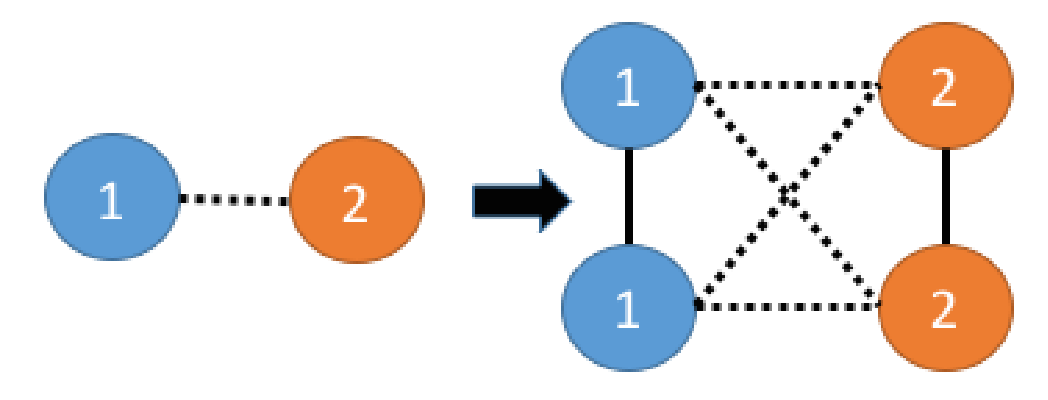
\includegraphics[width=0.5\columnwidth]{figures/resilience.eps}}
	\subfloat[Link Isolation]{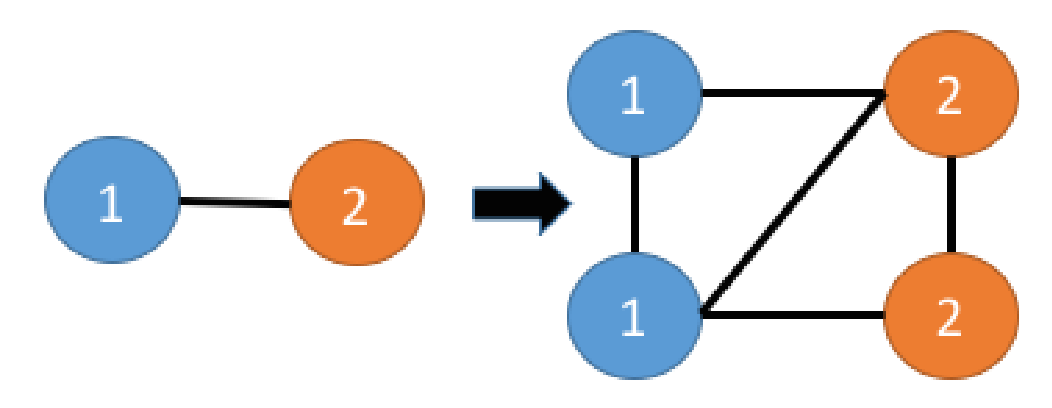
\includegraphics[width=0.5\columnwidth]{figures/resilience-cex.eps}}
	\caption{\label{fig:restransform}
		(a) Resilience Transformation for $pc_1 || \ pc_2$ for providing $1-resilience$. 
		The dotted lines represent traffic isolation policies, 
		while the solid lines represent link isolation. (b) Example of a sufficient transformation
		for 1-resilience in the case of a link-isolation policy.}
\end{figure}

\kausik{We can write something like TE with FFC, capacity policies such that
	the network is not congested in any failure scenario.}
We presented a sound transformation of policies to provide $t-resilience$ in
the case of reachability, waypoint and isolation policies. However, for global policies like 
traffic engineering, $t-resilience$ synthesis is complicated as the backup paths 
cannot be considered simply as different packet classes (they do not exist at the same time
in the network),
and thus cannot be considered in the optimization objective. Therefore, we require a 
temporal notion of the objective (like average link utilization) across link failures.
 Synthesis of resilient paths
satisfying traffic engineering objectives is one of the future directions of research.